% ============================================================================
%  VAE-Based Image Inpainting: A Research Survey and Architectural Proposal
%  for the FlowerPower Project
% ============================================================================
\documentclass[11pt, a4paper]{article}

% --- Typography & Layout ---
\usepackage[T1]{fontenc}
\usepackage{lmodern}
\usepackage{microtype}
\usepackage[margin=2.4cm, top=2.8cm, bottom=2.8cm]{geometry}
\usepackage{setspace}
\onehalfspacing

% --- Mathematics ---
\usepackage{amsmath, amssymb, amsthm, mathtools}
\newtheorem{definition}{Definition}
\newtheorem{remark}{Remark}

% --- Graphics & Figures ---
\usepackage{graphicx}
\usepackage{tikz}
\usetikzlibrary{positioning, arrows.meta, calc, fit, backgrounds, shapes.geometric}
\usepackage{pgfplots}
\pgfplotsset{compat=1.18}

% --- Tables ---
\usepackage{booktabs}
\usepackage{array}
\usepackage{multirow}
\usepackage{makecell}
\renewcommand\theadfont{\bfseries\small}

% --- Code listings ---
\usepackage{listings}
\lstset{
  language=Python,
  basicstyle=\ttfamily\footnotesize,
  keywordstyle=\bfseries\color[rgb]{0.13,0.29,0.53},
  stringstyle=\color[rgb]{0.31,0.54,0.16},
  commentstyle=\itshape\color{gray},
  backgroundcolor=\color[rgb]{0.97,0.97,0.97},
  frame=single,
  rulecolor=\color[rgb]{0.80,0.80,0.80},
  numbers=left,
  numberstyle=\tiny\color{gray},
  breaklines=true,
  captionpos=b,
  aboveskip=1em,
  belowskip=1em,
}

% --- Colours ---
\usepackage[dvipsnames]{xcolor}
\definecolor{secblue}{RGB}{30, 70, 130}
\definecolor{linkblue}{RGB}{0, 80, 160}
\definecolor{boxgray}{RGB}{245, 245, 245}
\definecolor{boxyellow}{RGB}{255, 252, 235}
\definecolor{boxgreen}{RGB}{237, 250, 240}
\definecolor{boxred}{RGB}{255, 240, 240}
\definecolor{boxpurple}{RGB}{243, 237, 255}

% --- Hyperlinks ---
\usepackage[colorlinks=true, linkcolor=linkblue, citecolor=linkblue, urlcolor=linkblue]{hyperref}

% --- Bibliography ---
\usepackage[numbers, sort&compress]{natbib}

% --- Miscellaneous ---
\usepackage{enumitem}
\usepackage{tcolorbox}
\tcbuselibrary{skins, breakable}
\usepackage{caption}
\captionsetup{font=small, labelfont=bf, skip=6pt}
\usepackage{fancyhdr}
\usepackage{titlesec}
\usepackage{algorithm}
\usepackage{algorithmic}

% --- Section Styling ---
\titleformat{\section}
  {\Large\bfseries\color{secblue}}{\thesection}{1em}{}[\vspace{2pt}\color{secblue}\hrule height 0.6pt]
\titleformat{\subsection}
  {\large\bfseries\color{secblue!80!black}}{\thesubsection}{0.8em}{}
\titleformat{\subsubsection}
  {\normalsize\bfseries\color{secblue!60!black}}{\thesubsubsection}{0.6em}{}

% --- Header/Footer ---
\pagestyle{fancy}
\fancyhf{}
\fancyhead[L]{\small\textit{VAE-Based Image Inpainting Research}}
\fancyhead[R]{\small\textit{FlowerPower Project}}
\fancyfoot[C]{\thepage}
\renewcommand{\headrulewidth}{0.4pt}

% --- Colored Boxes ---
\newtcolorbox{keyinsight}[1][]{
  colback=boxgreen, colframe=green!50!black,
  fonttitle=\bfseries, title={Key Insight}, #1
}
\newtcolorbox{warningbox}[1][]{
  colback=boxred, colframe=red!60!black,
  fonttitle=\bfseries, title={Warning}, #1
}
\newtcolorbox{notebox}[1][]{
  colback=boxyellow, colframe=orange!60!black,
  fonttitle=\bfseries, title={Note}, #1
}
\newtcolorbox{graybox}[1][]{
  colback=boxgray, colframe=gray!50!black,
  fonttitle=\bfseries, #1
}
\newtcolorbox{readybox}[1][]{
  colback=boxpurple, colframe=violet!60!black,
  fonttitle=\bfseries, title={Ready to Use}, #1
}

% --- Custom commands ---
\newcommand{\loss}{\mathcal{L}}
\newcommand{\KL}{\mathrm{KL}}
\newcommand{\ELBO}{\mathrm{ELBO}}
\newcommand{\reals}{\mathbb{R}}
\newcommand{\E}{\mathbb{E}}
\newcommand{\N}{\mathcal{N}}

% ============================================================================
\begin{document}

% --- Title Block ---
\begin{center}
  {\color{secblue}\rule{\textwidth}{1.2pt}}\\[0.8em]
  {\LARGE\bfseries\color{secblue} VAE-Based Image Inpainting}\\[0.3em]
  {\LARGE\bfseries\color{secblue} A Research Survey and Architectural Proposal}\\[0.6em]
  {\color{secblue}\rule{\textwidth}{1.2pt}}\\[1.2em]
  {\large\textit{FlowerPower Project --- Internal Research Document}}\\[0.5em]
  {\normalsize\today}
\end{center}

\vspace{1.5em}

% --- Abstract ---
\begin{abstract}
\noindent
The FlowerPower project currently compares two generative approaches for image inpainting on 128\(\times\)128 flower images: a custom U-Net GAN trained from scratch and a fine-tuned LaMa (Large Mask Inpainting) model based on Fast Fourier Convolutions. This document investigates the feasibility of introducing a Variational Autoencoder (VAE) based paradigm to the comparison. We organise our findings into two categories: (i)~\textbf{inference-ready models} with pre-trained weights that can be applied directly to the flower images without architectural changes or full retraining, and (ii)~\textbf{models requiring retraining} that need architectural adaptation or training from scratch. For the inference-ready category, we identify the Diverse Structure Inpainting model (hierarchical VQ-VAE) and the ICT/PUT transformer-based approaches with VQ-VAE tokenisers. (Note: Stable Diffusion was considered but dropped due to prohibitive inference times on CPU hardware). For the retraining category, we survey VAEAC, propose a custom convolutional VAE--GAN hybrid, and discuss training strategies including KL annealing and adversarial sharpening.
\end{abstract}

\tableofcontents
\newpage

% ============================================================================
\section{Introduction and Motivation}
% ============================================================================

The FlowerPower project addresses the problem of \textbf{image inpainting}---reconstructing missing or corrupted regions of an image given the surrounding context. The project operates on the Oxford 102 Flowers dataset, resized to \(128 \times 128\) pixels, with large contiguous masks (halves, quadrants, and large random rectangles covering 30--70\% of the image).

Two generative approaches are currently implemented:

\begin{enumerate}[leftmargin=2em]
  \item \textbf{U-Net GAN} (\texttt{GAN\_implementation/}): A custom encoder--decoder generator with skip connections, trained adversarially with a PatchGAN-style discriminator.
  \item \textbf{LaMa Fine-Tuning} (\texttt{lama\_finetuning/}): Fine-tuning of the state-of-the-art LaMa model, which uses Fast Fourier Convolutions (FFCs) for image-wide receptive fields.
\end{enumerate}

Both approaches share a common infrastructure defined in \texttt{shared\_utils.py}: the \texttt{ImageDataset}, \texttt{Discriminator}, \texttt{get\_large\_random\_mask}, and \texttt{compute\_gradient\_loss} utilities. Adding a \textbf{Variational Autoencoder (VAE)} based approach introduces a fundamentally different generative paradigm based on probabilistic latent-variable modelling, enabling a principled three-way comparison across architectural philosophies.

\begin{keyinsight}
A VAE offers something neither the GAN nor LaMa provides: a \emph{structured, interpretable latent space} learned via variational inference. This enables probabilistic reasoning about the inpainted output (e.g., sampling multiple plausible completions) and provides a theoretically grounded training objective (the ELBO), which avoids the mode collapse and training instability common in adversarial training.
\end{keyinsight}


% ============================================================================
\section{Mathematical Foundations of VAEs}
\label{sec:vae_foundations}
% ============================================================================

\subsection{The Generative Model and Variational Inference}

A Variational Autoencoder~\cite{kingma2014vae, reznik2014vae} posits a latent-variable generative model of the form:
\begin{equation}
  p_\theta(\mathbf{x}) = \int p_\theta(\mathbf{x} \mid \mathbf{z})\, p(\mathbf{z})\, d\mathbf{z},
  \label{eq:generative_model}
\end{equation}
where \(\mathbf{x} \in \reals^D\) is the observed data (an image), \(\mathbf{z} \in \reals^d\) is a latent representation, \(p(\mathbf{z}) = \N(\mathbf{0}, \mathbf{I})\) is the prior, and \(p_\theta(\mathbf{x} \mid \mathbf{z})\) is the decoder (likelihood) parameterised by a neural network with weights~\(\theta\).

Since the true posterior \(p_\theta(\mathbf{z} \mid \mathbf{x})\) is intractable, we introduce an \textbf{approximate posterior} (encoder):
\begin{equation}
  q_\phi(\mathbf{z} \mid \mathbf{x}) = \N\!\big(\boldsymbol{\mu}_\phi(\mathbf{x}),\; \mathrm{diag}\!\big(\boldsymbol{\sigma}_\phi^2(\mathbf{x})\big)\big),
  \label{eq:encoder}
\end{equation}
where \(\boldsymbol{\mu}_\phi\) and \(\boldsymbol{\sigma}_\phi^2\) are outputs of the encoder network.

\subsection{The Evidence Lower Bound (ELBO)}

Training maximises the Evidence Lower Bound on the log-likelihood:
\begin{equation}
  \boxed{
    \log p_\theta(\mathbf{x}) \;\geq\; \ELBO(\theta, \phi; \mathbf{x})
    \;=\; \underbrace{\E_{q_\phi(\mathbf{z} \mid \mathbf{x})}\!\big[\log p_\theta(\mathbf{x} \mid \mathbf{z})\big]}_{\text{Reconstruction term}}
    \;-\; \underbrace{\KL\!\big(q_\phi(\mathbf{z} \mid \mathbf{x}) \,\|\, p(\mathbf{z})\big)}_{\text{Regularisation term}}
  }
  \label{eq:elbo}
\end{equation}

The \textbf{reconstruction term} encourages the decoder to faithfully reproduce the input from its latent code. The \textbf{KL divergence term} regularises the latent space to stay close to the standard normal prior, enabling smooth interpolation and meaningful sampling.

\subsection{The Reparameterisation Trick}

To enable gradient-based optimisation through the stochastic sampling step, the reparameterisation trick~\cite{kingma2014vae} expresses the latent sample as a deterministic, differentiable function of the encoder outputs and an auxiliary noise variable:
\begin{equation}
  \mathbf{z} = \boldsymbol{\mu}_\phi(\mathbf{x}) + \boldsymbol{\sigma}_\phi(\mathbf{x}) \odot \boldsymbol{\epsilon}, \qquad \boldsymbol{\epsilon} \sim \N(\mathbf{0}, \mathbf{I}).
  \label{eq:reparam}
\end{equation}

\subsection{Adaptation to Conditional Inpainting}
\label{sec:cvae}

For inpainting, the model must be \textbf{conditioned} on the observed (unmasked) context. Given a masked image \(\mathbf{x}_{\text{masked}}\) and a binary mask \(\mathbf{m}\), we define a \textbf{Conditional VAE (CVAE)}~\cite{sohn2015cvae} whose encoder and decoder both receive the conditioning information:
\begin{align}
  q_\phi(\mathbf{z} \mid \mathbf{x}, \mathbf{c}) &= \N\!\big(\boldsymbol{\mu}_\phi(\mathbf{x}, \mathbf{c}),\; \mathrm{diag}\!\big(\boldsymbol{\sigma}_\phi^2(\mathbf{x}, \mathbf{c})\big)\big), \label{eq:cvae_encoder} \\[4pt]
  p_\theta(\mathbf{x} \mid \mathbf{z}, \mathbf{c}) &= \text{Decoder}_\theta(\mathbf{z}, \mathbf{c}), \label{eq:cvae_decoder}
\end{align}
where \(\mathbf{c} = [\mathbf{x}_{\text{masked}};\, \mathbf{m}]\) is the 4-channel conditioning input (identical to the input format already used by the U-Net GAN and LaMa in the FlowerPower project).

\subsection{Discrete Latent Spaces: VQ-VAE}
\label{sec:vqvae}

An important variant replaces the continuous Gaussian latent space with a \textbf{discrete codebook}. The Vector Quantised VAE (VQ-VAE)~\cite{oord2017vqvae} learns a codebook \(\mathbf{e} = \{e_1, \ldots, e_K\} \subset \reals^d\) and maps each encoder output to its nearest codebook entry:
\begin{equation}
  \mathbf{z}_q = e_k, \quad \text{where} \quad k = \arg\min_j \| \mathbf{z}_e - e_j \|_2.
  \label{eq:vqvae}
\end{equation}

The training loss combines reconstruction, codebook, and commitment terms:
\begin{equation}
  \loss_{\text{VQ-VAE}} = \| \mathbf{x} - \hat{\mathbf{x}} \|_2^2 + \| \mathrm{sg}[\mathbf{z}_e] - \mathbf{z}_q \|_2^2 + \beta \| \mathbf{z}_e - \mathrm{sg}[\mathbf{z}_q] \|_2^2,
  \label{eq:vqvae_loss}
\end{equation}
where $\mathrm{sg}[\cdot]$ denotes the stop-gradient operator.

VQ-VAEs are relevant to inpainting because they enable autoregressive generation of discrete tokens conditioned on context---a strategy exploited by several inference-ready models surveyed below.

\begin{notebox}
During \textbf{training}, the encoder sees the \emph{complete} ground-truth image concatenated with the conditioning context, while the decoder receives only the latent code and the conditioning context. During \textbf{inference}, the encoder receives only the masked image and context (or the conditioning is passed directly to the decoder), and the decoder produces the inpainted output.
\end{notebox}


% ============================================================================
\section{Inference-Ready VAE-Based Models}
\label{sec:ready}
% ============================================================================

This section surveys models that include \textbf{pre-trained weights} and can be applied to the flower images \textbf{without architectural modifications or full retraining}. Some require upscaling images from \(128 \times 128\) to \(256 \times 256\) or \(512 \times 512\), which is an acceptable pre-processing step.




\subsection{Diverse Structure Inpainting (Hierarchical VQ-VAE)}
\label{sec:dsi}

The \textbf{Diverse Structure Inpainting (DSI)} model~\cite{peng2021diverse} uses a hierarchical VQ-VAE to disentangle structure and texture for inpainting. It was published at CVPR 2021 and provides pre-trained checkpoints.

\subsubsection{Architecture Overview}

The model operates in two stages:
\begin{enumerate}[leftmargin=2em]
  \item \textbf{Structure Generator:} A hierarchical VQ-VAE encodes the image into a discrete token grid. An autoregressive transformer then generates tokens for the masked region, conditioned on the visible tokens. This produces diverse coarse structural completions.
  \item \textbf{Texture Generator:} A GAN-based refinement network adds high-fidelity texture details to the coarse structural output.
\end{enumerate}

\subsubsection{Suitability Assessment}

\begin{table}[H]
\centering
\caption{Diverse Structure Inpainting suitability assessment.}
\label{tab:dsi_suit}
\begin{tabular}{@{} >{\raggedright\arraybackslash}p{3.2cm} p{9.5cm} @{}}
\toprule
\thead{Criterion} & \thead{Assessment} \\
\midrule
Ready to use? & \textbf{Yes} --- checkpoints available for CelebA-HQ and Places2 \\
\addlinespace
Native resolution & \(256 \times 256\) (upscale from \(128 \times 128\) required) \\
\addlinespace
VAE role & Central: the hierarchical VQ-VAE is the backbone for structure representation and diverse generation \\
\addlinespace
Diversity & \textbf{Excellent} --- can sample multiple structurally different completions via different autoregressive token sequences \\
\addlinespace
Inference speed & \textbf{Slow}: $\sim$45 seconds per image on an NVIDIA 1080 Ti due to autoregressive token-by-token generation (can be improved with incremental sampling) \\
\addlinespace
Domain gap & Pre-trained on faces (CelebA-HQ) or scenes (Places2), \textbf{not flowers}. Results may show domain-specific artefacts \\
\bottomrule
\end{tabular}
\end{table}

\begin{graybox}[title={Reference Implementation}]
\textbf{Repository:} \texttt{USTC-JialunPeng/Diverse-Structure-Inpainting} (PyTorch) \\
\textbf{Paper:} Peng et al., ``Generating Diverse Structure for Image Inpainting With Hierarchical VQ-VAE,'' CVPR 2021 \\
\textbf{Checkpoints:} CelebA-HQ and Places2 available via repository README
\end{graybox}

\begin{warningbox}
The pre-trained checkpoints were trained on \textbf{faces} and \textbf{scenes}, not flowers. While the model will run without errors, the generated structures will likely reflect the training domain (e.g., face-like or scene-like textures in the filled region). This makes it a useful \emph{baseline} but not an ideal domain-matched comparison.
\end{warningbox}


\subsection{ICT: Image Completion Transformer with VQ-VAE}
\label{sec:ict}

The \textbf{Image Completion Transformer (ICT)}~\cite{wan2021ict} uses a two-stage VQ-VAE + Transformer pipeline for pluralistic (diverse) image inpainting. It was published at ICCV 2021.

\subsubsection{Architecture Overview}

\begin{enumerate}[leftmargin=2em]
  \item \textbf{VQ-VAE Tokeniser:} Encodes the image into a grid of discrete tokens using a learned codebook.
  \item \textbf{Bidirectional Transformer:} Iteratively predicts tokens for masked positions, conditioned on visible tokens, enabling diverse completions.
  \item \textbf{Guided Upsampler:} Refines the coarse VQ-VAE reconstruction to full resolution.
\end{enumerate}

\subsubsection{Suitability Assessment}

\begin{table}[H]
\centering
\caption{ICT suitability assessment.}
\label{tab:ict_suit}
\begin{tabular}{@{} >{\raggedright\arraybackslash}p{3.2cm} p{9.5cm} @{}}
\toprule
\thead{Criterion} & \thead{Assessment} \\
\midrule
Ready to use? & \textbf{Yes} --- checkpoints downloadable (Dropbox/OneDrive/Baidu) \\
\addlinespace
Native resolution & \(256 \times 256\) (upscale from \(128 \times 128\) required) \\
\addlinespace
VAE role & Central: VQ-VAE tokeniser converts images to/from discrete tokens \\
\addlinespace
Diversity & \textbf{Excellent} --- multiple completions via stochastic token sampling \\
\addlinespace
Domain gap & Trained on FFHQ and Places2; same domain gap caveat as DSI \\
\bottomrule
\end{tabular}
\end{table}

\begin{graybox}[title={Reference Implementation}]
\textbf{Repository:} \texttt{raywzy/ICT} (PyTorch) \\
\textbf{Paper:} Wan et al., ``High-Fidelity Pluralistic Image Completion with Transformers,'' ICCV 2021
\end{graybox}


\subsection{PUT: Pluralistic Image Completion with Reduced Information Loss}
\label{sec:put}

\textbf{PUT}~\cite{liu2022put} extends ICT by addressing the information loss caused by aggressive quantisation in VQ-VAE tokenisation. It uses an improved ``un-quantised transformer'' approach that operates on continuous features rather than discrete tokens, yielding sharper results.

\begin{table}[H]
\centering
\caption{PUT suitability assessment.}
\label{tab:put_suit}
\begin{tabular}{@{} >{\raggedright\arraybackslash}p{3.2cm} p{9.5cm} @{}}
\toprule
\thead{Criterion} & \thead{Assessment} \\
\midrule
Ready to use? & \textbf{Yes} --- checkpoints available via \texttt{liuqk3/PUT} on GitHub \\
\addlinespace
Native resolution & \(256 \times 256\) \\
\addlinespace
Key improvement & Reduces quantisation artefacts by operating on continuous VQ-VAE features \\
\addlinespace
Domain gap & Same caveat: pre-trained on FFHQ and Places2 \\
\bottomrule
\end{tabular}
\end{table}

\begin{graybox}[title={Reference Implementation}]
\textbf{Repository:} \texttt{liuqk3/PUT} (PyTorch) \\
\textbf{Paper:} Liu et al., ``Reduce Information Loss in Transformers for Pluralistic Image Inpainting,'' CVPR 2022
\end{graybox}


\subsection{Summary of Inference-Ready Models}

\begin{table}[H]
\centering
\caption{Comparative summary of inference-ready VAE-based inpainting models.}
\label{tab:ready_summary}
\renewcommand{\arraystretch}{1.2}
\begin{tabular}{@{} l c c c c c @{}}
\toprule
\thead{Model} & \thead{VAE\\Type} & \thead{Native\\Res.} & \thead{Diverse?} & \thead{Domain\\Match} & \thead{Quality} \\
\midrule
SD Inpainting & KL-VAE & $512^2$ & No & \textbf{Good} (general) & \textbf{Excellent} \\
DSI & hier.~VQ-VAE & $256^2$ & \textbf{Yes} & Poor (faces/scenes) & Good \\
ICT & VQ-VAE & $256^2$ & \textbf{Yes} & Poor (faces/scenes) & Good \\
PUT & VQ-VAE+ & $256^2$ & \textbf{Yes} & Poor (faces/scenes) & Good+ \\
\bottomrule
\end{tabular}
\end{table}

\begin{keyinsight}
\textbf{Recommended inference-ready approach:} For showcasing the \textbf{diversity} advantage of VAE latent spaces (multiple plausible completions), \textbf{PUT} or \textbf{ICT} are the best choices---though their domain gap with flower images should be acknowledged.
\end{keyinsight}


% ============================================================================
\section{Models Requiring Retraining or Architectural Changes}
\label{sec:retrain}
% ============================================================================

This section covers models that require either \textbf{significant architectural modifications} to handle \(128 \times 128\) flower images, or \textbf{full training from scratch} on the flower dataset. These approaches offer tighter integration with the FlowerPower codebase and fairer comparisons, at the cost of implementation and training effort.

\subsection{VAEAC: VAE with Arbitrary Conditioning}
\label{sec:vaeac}

\textbf{VAEAC}~\cite{ivanov2019vaeac} is the most directly relevant pure-VAE model for inpainting. It extends the standard CVAE framework to condition on an \textit{arbitrary} subset of observed features, making it a natural fit for inpainting where the ``observed subset'' is defined by the mask.

\subsubsection{Architecture}

VAEAC introduces three key networks:
\begin{itemize}[leftmargin=1.5em]
  \item A \textbf{proposal network} \(q_\phi(\mathbf{z} \mid \mathbf{x}, \mathbf{b})\): encodes the full observation with knowledge of which features are observed.
  \item A \textbf{prior network} \(p_\psi(\mathbf{z} \mid \mathbf{x}_{\text{obs}}, \mathbf{b})\): produces a \emph{conditional prior} from only the observed features, replacing the fixed \(\N(\mathbf{0}, \mathbf{I})\) prior.
  \item A \textbf{generative network} \(p_\theta(\mathbf{x}_{\text{miss}} \mid \mathbf{z}, \mathbf{x}_{\text{obs}}, \mathbf{b})\): decodes the missing features.
\end{itemize}

The modified ELBO becomes:
\begin{equation}
  \loss_{\text{VAEAC}} = -\E_{q_\phi}\!\big[\log p_\theta(\mathbf{x}_{\text{miss}} \mid \mathbf{z}, \mathbf{x}_{\text{obs}}, \mathbf{b})\big] + \KL\!\big(q_\phi(\mathbf{z} \mid \mathbf{x}, \mathbf{b}) \,\|\, p_\psi(\mathbf{z} \mid \mathbf{x}_{\text{obs}}, \mathbf{b})\big).
  \label{eq:vaeac_loss}
\end{equation}

\subsubsection{Why It Cannot Be Used Directly}

\begin{table}[H]
\centering
\caption{VAEAC barriers to direct use.}
\label{tab:vaeac_barriers}
\begin{tabular}{@{} >{\raggedright\arraybackslash}p{3.5cm} p{9cm} @{}}
\toprule
\thead{Barrier} & \thead{Detail} \\
\midrule
Architecture mismatch & Published code uses \textbf{fully-connected layers}; must be rewritten with convolutional encoder/decoder for \(128 \times 128\) images \\
\addlinespace
No pre-trained weights & Demonstrated only on MNIST (\(28 \times 28\)) and tabular data; no weights for natural images exist \\
\addlinespace
Full retraining & Requires complete training on the flower dataset from scratch \\
\bottomrule
\end{tabular}
\end{table}

\begin{graybox}[title={Reference Implementation}]
\textbf{Repository:} \texttt{tigvarts/vaeac} (PyTorch) \\
\textbf{Paper:} Ivanov et al., ``Variational Autoencoder with Arbitrary Conditioning,'' ICLR 2019
\end{graybox}


\subsection{Stable Diffusion VAE Standalone (AutoencoderKL)}
\label{sec:sd_vae_standalone}

The Stable Diffusion VAE (\texttt{AutoencoderKL} from \texttt{diffusers}) is a powerful pre-trained encoder/decoder, but using it \textbf{alone} (without the diffusion U-Net) for inpainting is problematic.

\begin{warningbox}
Using the SD VAE alone (without the diffusion backbone) is unconventional and \textbf{not recommended}. The VAE was designed as a compression stage, not a standalone generator. Without the diffusion U-Net to guide generation in masked regions, the VAE decoder simply reconstructs whatever latent it receives---producing blurry, semantically incoherent results in masked areas. This would not reflect the VAE paradigm fairly.
\end{warningbox}

\subsection{Proposed Custom Architecture: Convolutional VAE--GAN}
\label{sec:proposed}

Given the limitations of existing models, we propose building a \textbf{custom convolutional VAE--GAN hybrid} that integrates directly with the FlowerPower codebase.

\subsubsection{Design Principles}

\begin{enumerate}[leftmargin=2em]
  \item \textbf{Same input/output format}: 4-channel input \([\mathbf{x}_{\text{masked}} \oplus \mathbf{m}]\), 3-channel output in \([-1, 1]\) via \(\tanh\).
  \item \textbf{Same composition}: The output is composited as \(\mathbf{x}_{\text{comp}} = \mathbf{x}_{\text{masked}} + \hat{\mathbf{x}} \odot \mathbf{m}\).
  \item \textbf{Same adversarial framework}: Reuses the shared \texttt{Discriminator} for adversarial training.
  \item \textbf{Same evaluation pipeline}: Compatible with the existing \texttt{evaluate.py} visualisation code.
\end{enumerate}

\subsubsection{Architecture Diagram}

\begin{figure}[H]
\centering
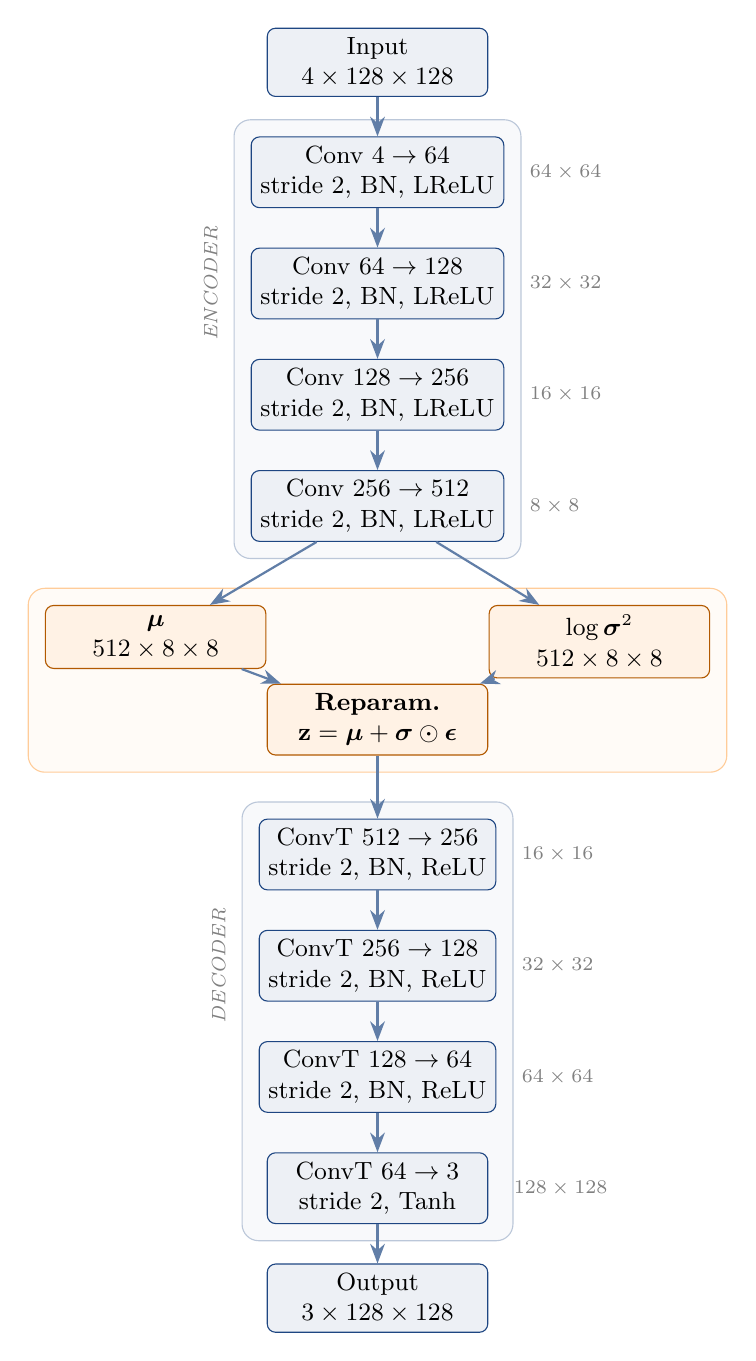
\begin{tikzpicture}[
    block/.style={rectangle, draw=secblue, fill=secblue!8, rounded corners=3pt,
                  minimum width=2.8cm, minimum height=0.8cm, align=center,
                  font=\small},
    latent/.style={rectangle, draw=orange!70!black, fill=orange!10, rounded corners=3pt,
                  minimum width=2.8cm, minimum height=0.8cm, align=center,
                  font=\small},
    arr/.style={-{Stealth[length=2.5mm]}, thick, color=secblue!70},
    label/.style={font=\scriptsize\itshape, text=gray}
  ]
  % Encoder
  \node[block] (in) {Input\\$4 \times 128 \times 128$};
  \node[block, below=0.5cm of in] (e1) {Conv $4 \to 64$\\stride 2, BN, LReLU};
  \node[block, below=0.5cm of e1] (e2) {Conv $64 \to 128$\\stride 2, BN, LReLU};
  \node[block, below=0.5cm of e2] (e3) {Conv $128 \to 256$\\stride 2, BN, LReLU};
  \node[block, below=0.5cm of e3] (e4) {Conv $256 \to 512$\\stride 2, BN, LReLU};

  % Latent
  \node[latent, below left=0.8cm and -0.2cm of e4] (mu) {$\boldsymbol{\mu}$\\$512 \times 8 \times 8$};
  \node[latent, below right=0.8cm and -0.2cm of e4] (logvar) {$\log\boldsymbol{\sigma}^2$\\$512 \times 8 \times 8$};
  \node[latent, below=1.8cm of e4] (z) {\textbf{Reparam.}\\$\mathbf{z} = \boldsymbol{\mu} + \boldsymbol{\sigma} \odot \boldsymbol{\epsilon}$};

  % Decoder
  \node[block, below=0.8cm of z] (d1) {ConvT $512 \to 256$\\stride 2, BN, ReLU};
  \node[block, below=0.5cm of d1] (d2) {ConvT $256 \to 128$\\stride 2, BN, ReLU};
  \node[block, below=0.5cm of d2] (d3) {ConvT $128 \to 64$\\stride 2, BN, ReLU};
  \node[block, below=0.5cm of d3] (d4) {ConvT $64 \to 3$\\stride 2, Tanh};
  \node[block, below=0.5cm of d4] (out) {Output\\$3 \times 128 \times 128$};

  % Labels
  \node[label, left=0.3cm of e2] (elabel) {\rotatebox{90}{ENCODER}};
  \node[label, left=0.3cm of d2] (dlabel) {\rotatebox{90}{DECODER}};

  % Arrows
  \draw[arr] (in) -- (e1);
  \draw[arr] (e1) -- (e2);
  \draw[arr] (e2) -- (e3);
  \draw[arr] (e3) -- (e4);
  \draw[arr] (e4) -- (mu);
  \draw[arr] (e4) -- (logvar);
  \draw[arr] (mu) -- (z);
  \draw[arr] (logvar) -- (z);
  \draw[arr] (z) -- (d1);
  \draw[arr] (d1) -- (d2);
  \draw[arr] (d2) -- (d3);
  \draw[arr] (d3) -- (d4);
  \draw[arr] (d4) -- (out);

  % Spatial dims
  \node[label, right=0.2cm of e1] {$64 \times 64$};
  \node[label, right=0.2cm of e2] {$32 \times 32$};
  \node[label, right=0.2cm of e3] {$16 \times 16$};
  \node[label, right=0.2cm of e4] {$8 \times 8$};
  \node[label, right=0.2cm of d1] {$16 \times 16$};
  \node[label, right=0.2cm of d2] {$32 \times 32$};
  \node[label, right=0.2cm of d3] {$64 \times 64$};
  \node[label, right=0.2cm of d4] {$128 \times 128$};

  % Bounding boxes
  \begin{scope}[on background layer]
    \node[fit=(e1)(e4), draw=secblue!30, fill=secblue!3, rounded corners=6pt, inner sep=6pt] {};
    \node[fit=(d1)(d4), draw=secblue!30, fill=secblue!3, rounded corners=6pt, inner sep=6pt] {};
    \node[fit=(mu)(logvar)(z), draw=orange!40, fill=orange!3, rounded corners=6pt, inner sep=6pt] {};
  \end{scope}
\end{tikzpicture}
\caption{Proposed \texttt{ConvVAEGenerator} architecture. The encoder compresses the 4-channel input into a spatial latent map at \(8 \times 8\) resolution. The reparameterisation trick samples from the learned distribution, and the decoder reconstructs the 3-channel output.}
\label{fig:architecture}
\end{figure}


\subsubsection{Detailed Layer Specification}

\begin{table}[H]
\centering
\caption{Detailed layer specification for the proposed \texttt{ConvVAEGenerator}.}
\label{tab:layer_spec}
\renewcommand{\arraystretch}{1.15}
\begin{tabular}{@{} c l l c c @{}}
\toprule
\thead{Stage} & \thead{Layer} & \thead{Configuration} & \thead{Output Shape} & \thead{Params} \\
\midrule
\multirow{4}{*}{\rotatebox{90}{\scriptsize Enc.}}
& Conv2d + BN + LReLU & \(4 \to 64\), \(k{=}4, s{=}2, p{=}1\) & \(64 \times 64 \times 64\) & 4.2K \\
& Conv2d + BN + LReLU & \(64 \to 128\), \(k{=}4, s{=}2, p{=}1\) & \(128 \times 32 \times 32\) & 131K \\
& Conv2d + BN + LReLU & \(128 \to 256\), \(k{=}4, s{=}2, p{=}1\) & \(256 \times 16 \times 16\) & 525K \\
& Conv2d + BN + LReLU & \(256 \to 512\), \(k{=}4, s{=}2, p{=}1\) & \(512 \times 8 \times 8\) & 2.1M \\
\midrule
\multirow{2}{*}{\rotatebox{90}{\scriptsize Lat.}}
& Conv2d (\(\boldsymbol{\mu}\)) & \(512 \to 512\), \(k{=}3, s{=}1, p{=}1\) & \(512 \times 8 \times 8\) & 2.4M \\
& Conv2d (\(\log\boldsymbol{\sigma}^2\)) & \(512 \to 512\), \(k{=}3, s{=}1, p{=}1\) & \(512 \times 8 \times 8\) & 2.4M \\
\midrule
\multirow{4}{*}{\rotatebox{90}{\scriptsize Dec.}}
& ConvT2d + BN + ReLU & \(512 \to 256\), \(k{=}4, s{=}2, p{=}1\) & \(256 \times 16 \times 16\) & 2.1M \\
& ConvT2d + BN + ReLU & \(256 \to 128\), \(k{=}4, s{=}2, p{=}1\) & \(128 \times 32 \times 32\) & 525K \\
& ConvT2d + BN + ReLU & \(128 \to 64\), \(k{=}4, s{=}2, p{=}1\) & \(64 \times 64 \times 64\) & 131K \\
& ConvT2d + Tanh & \(64 \to 3\), \(k{=}4, s{=}2, p{=}1\) & \(3 \times 128 \times 128\) & 3.1K \\
\midrule
\multicolumn{4}{@{}l}{\textbf{Total parameters}} & \(\approx\)\textbf{10.2M} \\
\bottomrule
\end{tabular}
\end{table}

\subsubsection{Training Objective: Hybrid VAE--GAN Loss}

The total generator loss combines the VAE-specific ELBO with the existing adversarial and perceptual losses:
\begin{equation}
  \boxed{
    \loss_{\text{total}} = \lambda_{\text{kl}}\, \loss_{\text{KL}}
                        + \lambda_{\text{L1}}\, \loss_{\text{L1}}
                        + \loss_{\text{adv}}
                        + \lambda_{\text{edge}}\, \loss_{\text{edge}}
                        + \lambda_{\text{perc}}\, \loss_{\text{perc}}
  }
  \label{eq:total_loss}
\end{equation}

where:
\begin{itemize}[leftmargin=1.5em]
  \item \(\loss_{\text{KL}}\): Closed-form KL divergence between the learned posterior and $\N(\mathbf{0}, \mathbf{I})$
  \item \(\loss_{\text{L1}}\): L1 pixel reconstruction loss on the masked region
  \item \(\loss_{\text{adv}}\): BCE adversarial loss via the shared \texttt{Discriminator}
  \item \(\loss_{\text{edge}}\): Gradient/edge loss from \texttt{compute\_gradient\_loss}
  \item \(\loss_{\text{perc}}\): VGG perceptual loss (optional, from \texttt{VGGPerceptualLoss})
\end{itemize}

Recommended weights: \(\lambda_{\text{kl}} = 0 \to 0.5\) (annealed over 5 epochs), \(\lambda_{\text{L1}} = 100\), \(\lambda_{\text{edge}} = 50\), \(\lambda_{\text{perc}} = 10\).


% ============================================================================
\section{Training Challenges and Mitigation Strategies}
\label{sec:challenges}
% ============================================================================

This section applies to models from Section~\ref{sec:retrain} that require training from scratch.

\subsection{Posterior Collapse}

\begin{definition}[Posterior Collapse]
Posterior collapse occurs when the approximate posterior $q_\phi(\mathbf{z} \mid \mathbf{x})$ collapses to the prior $p(\mathbf{z})$, i.e., $\KL(q_\phi \| p) \approx 0$, meaning the latent code carries no information about the input and the decoder learns to ignore~$\mathbf{z}$ entirely.
\end{definition}

\subsubsection{Mitigation: KL Annealing}

\textbf{KL annealing}~\cite{bowman2016kl_anneal} gradually increases the weight of the KL term during training:
\begin{equation}
  \lambda_{\text{kl}}(t) = \min\!\Big(\lambda_{\text{kl}}^{\max},\; \frac{t}{T_{\text{warmup}}} \cdot \lambda_{\text{kl}}^{\max}\Big)
  \label{eq:kl_anneal}
\end{equation}
where \(t\) is the current epoch and \(T_{\text{warmup}}\) is the warmup period.

\begin{figure}[H]
\centering
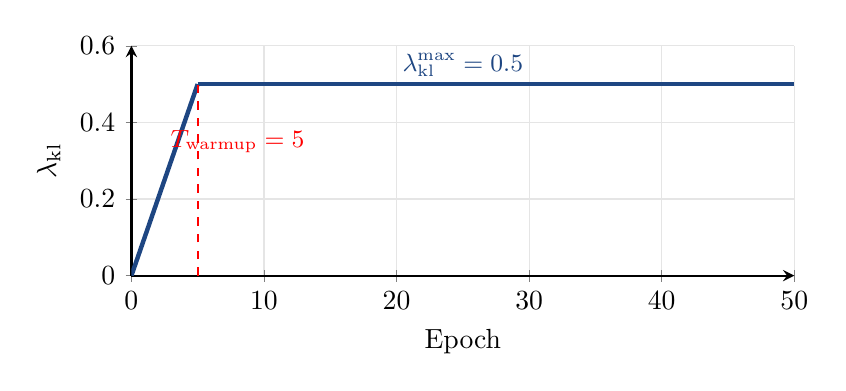
\begin{tikzpicture}
  \begin{axis}[
    width=10cm, height=4.5cm,
    xlabel={Epoch},
    ylabel={$\lambda_{\text{kl}}$},
    xmin=0, xmax=50, ymin=0, ymax=0.6,
    grid=major,
    grid style={gray!20},
    axis lines=left,
    thick,
  ]
  \addplot[color=secblue, ultra thick, domain=0:5] {0.5 * x / 5};
  \addplot[color=secblue, ultra thick, domain=5:50] {0.5};
  \addplot[color=red, dashed, thick] coordinates {(5, 0) (5, 0.5)};
  \node[font=\small, text=red] at (axis cs:8, 0.35) {$T_{\text{warmup}} = 5$};
  \node[font=\small, text=secblue] at (axis cs:25, 0.55) {$\lambda_{\text{kl}}^{\max} = 0.5$};
  \end{axis}
\end{tikzpicture}
\caption{KL annealing schedule: the KL weight increases linearly from 0 to \(\lambda_{\text{kl}}^{\max}\) over the first \(T_{\text{warmup}}\) epochs, then remains constant.}
\label{fig:kl_anneal}
\end{figure}

\subsubsection{Mitigation: Free Bits}

The \textbf{free bits} strategy~\cite{kingma2016freebits} sets a minimum threshold \(\lambda_{\text{fb}}\) for the per-dimension KL:
\begin{equation}
  \loss_{\text{KL}}^{\text{fb}} = \sum_{i} \max\!\Big(\lambda_{\text{fb}},\; \KL_i\big(q_\phi \| p\big)\Big)
  \label{eq:free_bits}
\end{equation}

\subsection{Blurriness}

\begin{keyinsight}
The hybrid VAE--GAN objective (Section~\ref{sec:proposed}) directly addresses blurriness through three complementary mechanisms:
\begin{enumerate}[leftmargin=1.5em]
  \item \textbf{Adversarial loss}: The discriminator penalises blurry outputs as ``fake.''
  \item \textbf{Gradient/edge loss}: Explicitly penalises loss of high-frequency detail.
  \item \textbf{VGG perceptual loss}: Enforces feature-level similarity rather than pixel-level averaging.
\end{enumerate}
These are the same tools already proven effective in the project's GAN and LaMa training.
\end{keyinsight}


% ============================================================================
\section{Expected Comparison Framework}
\label{sec:comparison}
% ============================================================================

\begin{table}[H]
\centering
\caption{Complete comparison of all surveyed approaches for flower inpainting.}
\label{tab:full_comparison}
\renewcommand{\arraystretch}{1.2}
\begin{tabular}{@{} l c c c c @{}}
\toprule
\thead{Model} & \thead{Category} & \thead{VAE Type} & \thead{Training\\Needed?} & \thead{Diverse?} \\
\midrule
U-Net GAN & Baseline & --- & Yes (done) & No \\
LaMa (FFC) & Baseline & --- & Fine-tune (done) & No \\
\midrule
DSI & Inference-ready & hier.~VQ-VAE & No & Yes \\
ICT & Inference-ready & VQ-VAE & No & Yes \\
PUT & Inference-ready & VQ-VAE+ & No & Yes \\
\midrule
VAEAC & Retrain & Conditional VAE & Full retrain & Yes \\
Custom ConvVAE & Retrain & KL-VAE + GAN & Full train & Yes \\
\bottomrule
\end{tabular}
\end{table}

\subsection{Evaluation Metrics}

For a fair comparison, all models should be evaluated with the same metrics on the same held-out test set:

\begin{enumerate}[leftmargin=2em]
  \item \textbf{L1 / L2 Error} (masked region): Pixel-level accuracy of the inpainted region.
  \item \textbf{PSNR}: Peak Signal-to-Noise Ratio of the composite image.
  \item \textbf{SSIM}: Structural Similarity Index capturing perceptual quality.
  \item \textbf{LPIPS}~\cite{zhang2018lpips}: Learned Perceptual Image Patch Similarity, which correlates better with human judgement than pixel-based metrics.
  \item \textbf{FID}~\cite{heusel2017fid}: Fr\'{e}chet Inception Distance on the composite images, measuring distributional similarity to real images.
\end{enumerate}

\begin{notebox}
Models that support \textbf{diverse completions} (DSI, ICT, PUT, VAEAC, Custom ConvVAE) can additionally be evaluated with a \textbf{diversity metric}: by sampling multiple completions for the same masked input and measuring the variance across them. This demonstrates the model's ability to represent the multimodal distribution of plausible inpaintings---a distinctive advantage of VAE-based latent spaces over deterministic approaches.
\end{notebox}


% ============================================================================
\section{Conclusion and Recommendations}
\label{sec:conclusion}
% ============================================================================

This document has surveyed the landscape of VAE-based approaches for image inpainting in the context of the FlowerPower project. Our findings are organised into two actionable categories:

\subsection*{For Immediate Results (No Training Required)}

\begin{enumerate}[leftmargin=2em]
    \item \textbf{PUT} or \textbf{ICT}: Best for demonstrating the diversity advantage of VAE latent spaces (multiple plausible completions). Upscale to \(256 \times 256\). Expect some domain gap artefacts since pre-trained on faces/scenes.
  \item \textbf{DSI}: Similar to ICT/PUT but with explicit structure/texture disentanglement. Slower inference ($\sim$45s/image).
\end{enumerate}

\subsection*{For a Fair, Controlled Comparison (Training Required)}

\begin{enumerate}[leftmargin=2em]
  \item \textbf{Custom ConvVAE--GAN hybrid} (recommended): Drops directly into the existing codebase, reuses all shared utilities, provides a fair three-way comparison with identical data pipelines, mask strategies, and discriminators.
  \item \textbf{VAEAC}: Academically interesting but requires significant re-engineering of the architecture from fully-connected to convolutional layers.
\end{enumerate}

\subsection*{Suggested Implementation Order}

\begin{enumerate}[leftmargin=2em]
    \item Run \textbf{PUT/ICT} to showcase diverse VAE-based completions.
  \item Implement and train the \textbf{custom ConvVAE--GAN} for the controlled comparison.
  \item Compile all results into a unified evaluation.
\end{enumerate}


% ============================================================================
% References
% ============================================================================
\begin{thebibliography}{20}

\bibitem{kingma2014vae}
D.~P. Kingma and M.~Welling,
``Auto-Encoding Variational Bayes,''
in \textit{Proc. ICLR}, 2014.

\bibitem{reznik2014vae}
D.~J. Rezende, S.~Mohamed, and D.~Wierstra,
``Stochastic Backpropagation and Approximate Inference in Deep Generative Models,''
in \textit{Proc. ICML}, pp.~1278--1286, 2014.

\bibitem{sohn2015cvae}
K.~Sohn, H.~Lee, and X.~Yan,
``Learning Structured Output Representation using Deep Conditional Generative Models,''
in \textit{Proc. NeurIPS}, pp.~3483--3491, 2015.

\bibitem{oord2017vqvae}
A.~van~den~Oord, O.~Vinyals, and K.~Kavukcuoglu,
``Neural Discrete Representation Learning,''
in \textit{Proc. NeurIPS}, pp.~6306--6315, 2017.

\bibitem{ivanov2019vaeac}
O.~Ivanov, M.~Figurnov, and D.~Vetrov,
``Variational Autoencoder with Arbitrary Conditioning,''
in \textit{Proc. ICLR}, 2019.

\bibitem{bowman2016kl_anneal}
S.~R. Bowman, L.~Vilnis, O.~Vinyals, A.~M. Dai, R.~Jozefowicz, and S.~Bengio,
``Generating Sentences from a Continuous Space,''
in \textit{Proc. CoNLL}, pp.~10--21, 2016.

\bibitem{kingma2016freebits}
D.~P. Kingma, T.~Salimans, R.~Jozefowicz, X.~Chen, I.~Sutskever, and M.~Welling,
``Improved Variational Inference with Inverse Autoregressive Flow,''
in \textit{Proc. NeurIPS}, pp.~4743--4751, 2016.

\bibitem{peng2021diverse}
J.~Peng, D.~Liu, S.~Xu, and H.~Li,
``Generating Diverse Structure for Image Inpainting With Hierarchical VQ-VAE,''
in \textit{Proc. CVPR}, pp.~10775--10784, 2021.

\bibitem{wan2021ict}
Z.~Wan, J.~Zhang, D.~Chen, and J.~Liao,
``High-Fidelity Pluralistic Image Completion with Transformers,''
in \textit{Proc. ICCV}, pp.~4692--4701, 2021.

\bibitem{liu2022put}
Q.~Liu, Z.~Tan, D.~Chen, Q.~Chu, X.~Dai, Y.~Chen, M.~Liu, L.~Yuan, and N.~Yu,
``Reduce Information Loss in Transformers for Pluralistic Image Inpainting,''
in \textit{Proc. CVPR}, pp.~11347--11357, 2022.

\bibitem{rombach2022ldm}
R.~Rombach, A.~Blattmann, D.~Lorenz, P.~Esser, and B.~Ommer,
``High-Resolution Image Synthesis with Latent Diffusion Models,''
in \textit{Proc. CVPR}, pp.~10684--10695, 2022.

\bibitem{suvorov2022lama}
R.~Suvorov et al.,
``Resolution-robust Large Mask Inpainting with Fourier Convolutions,''
in \textit{Proc. WACV}, pp.~2149--2159, 2022.

\bibitem{heusel2017fid}
M.~Heusel, H.~Ramsauer, T.~Unterthiner, B.~Nessler, and S.~Hochreiter,
``GANs Trained by a Two Time-Scale Update Rule Converge to a Local Nash Equilibrium,''
in \textit{Proc. NeurIPS}, pp.~6626--6637, 2017.

\bibitem{zhang2018lpips}
R.~Zhang, P.~Isola, A.~A. Efros, E.~Shechtman, and O.~Wang,
``The Unreasonable Effectiveness of Deep Features as a Perceptual Metric,''
in \textit{Proc. CVPR}, pp.~586--595, 2018.

\end{thebibliography}

\end{document}
